\section{电动势产生的机理}

    \subsection{界面电势差}

    在水合作用下,一部分金属离子可以离开金属进入水层之中。这会导致金属带负电,溶液带正电,如图\ref{fig:surface_E}所示。

    \begin{figure}[h]
        \centering
        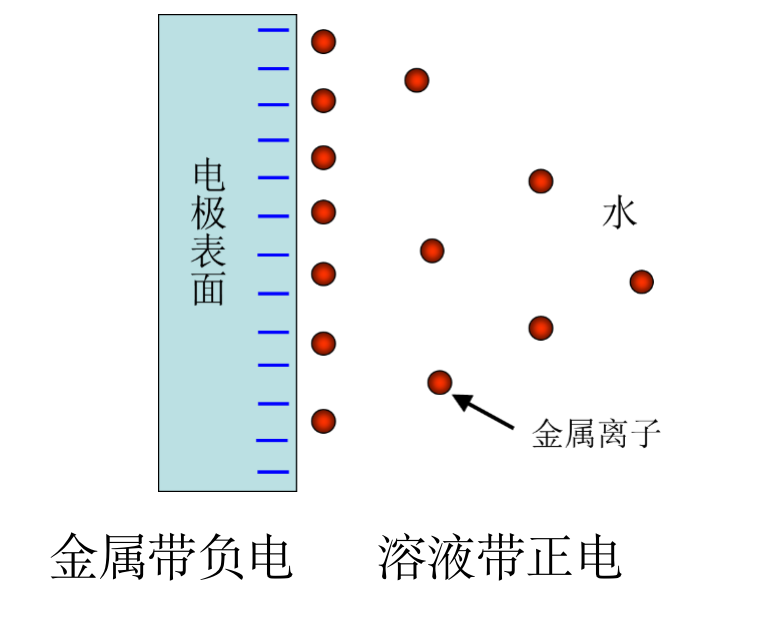
\includegraphics[width=0.6\textwidth]{surface_E.png}
        \caption{界面电势差的形成}
        \label{fig:surface_E}
    \end{figure}
    
    \subsubsection{紧密层}
    在金属与溶液的界面上,由于正、负离子静电吸引和热运动两种效应的结果,溶液中的金属离子只有一部分紧密地排在固体表面附近,相距约一、二个离子厚度。
    \subsubsection{扩散层}
    另一部分离子按一定的浓度梯度扩散到本体溶液中。

    \subsubsection{双电层}

    电极表面电荷层和溶液多余反离子构成\textbf{双电层}(见图\ref{fig:surface_E_layers})。金属表面和溶液本体之间的电势差即为界面电势差。

    
    \begin{figure}[h]
        \centering
        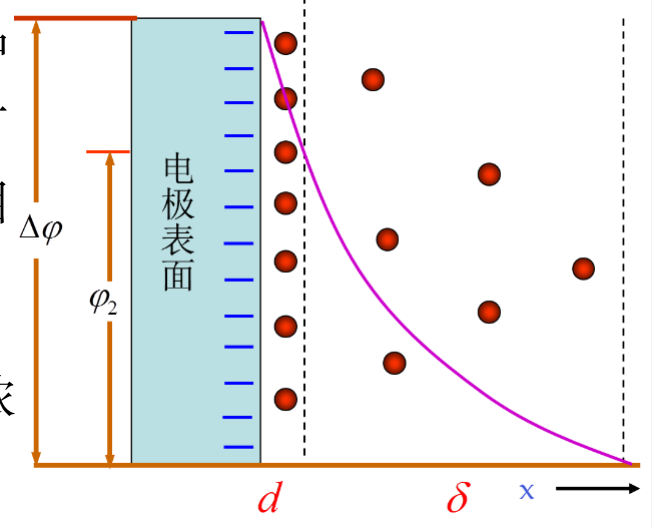
\includegraphics[width=0.6\textwidth]{surface_E_layers.png}
        \caption{紧密层-扩散层}
        \label{fig:surface_E_layers}
    \end{figure}


    

    \subsection{接触电势}

    电子逸出功,电子从金属表面逸出时,为了克服表面势垒所做的功。相互接触时,逸出功的大小不一致,导致表面间存在接触电势。


    \subsection{液体接界电势}

    在含有不同溶液的形成的界面上,或同一种溶液不同浓度所形成的的界面上,由于阴阳离子迁移的速度不一致,会导致界面形成微小的电动势。这一电动势被称为液接电势(图\ref{fig:ljp})。

    \begin{figure}[h]
        \centering
        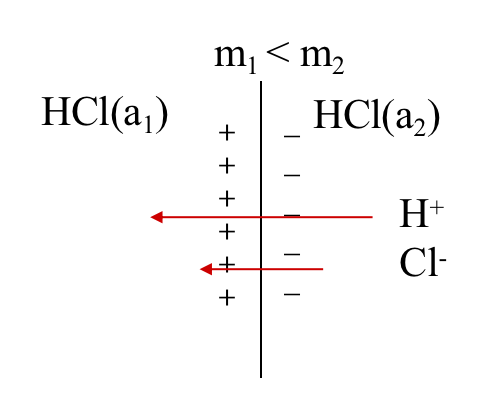
\includegraphics[width=0.6\textwidth]{ljp.png}
        \caption{液接电势的形成}
        \label{fig:ljp}
    \end{figure}

    \subsubsection{盐桥的作用}

    液接电势对电动势产生干扰,可以用\textbf{盐桥}(图\ref{fig:salt_bridge})来抵消液接电势。


    \begin{figure}[h]
        \centering
        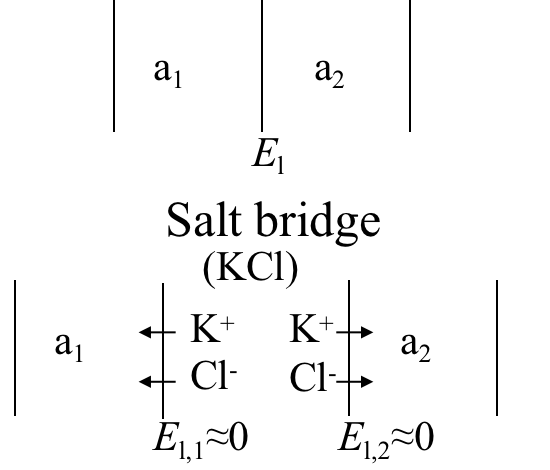
\includegraphics[width=0.6\textwidth]{salt_bridge.png}
        \caption{盐桥的作用}
        \label{fig:salt_bridge}
    \end{figure}

  